\task{Плавучий зоопарк}

\begin{itemize}
\itA Итак, мы знаем, что кобра спит, укусив себя за хвост и изогнувшись замкнутой ломаной. Например, ее положение может выглядеть так:

\begin{center} \tikz{
	\draw[very thick] (90:0.4) -- (210:1.3)
		-- (330:0.4) -- (90:1.3) -- (210:0.4) -- (330:1.3) -- cycle; 
} \end{center}

\itB \label{float-ptb} Конечно же, минимальное количество углов у пересечения~— 3. Если мы найдем максимальное количество и приведем пример, когда оно достигается, то все промежуточные количества углов будет несложно получить.

Покажем, что каждая сторона шестиугольника дает не более четырех углов будущему пересечению. Если концы этой стороны оба находятся снаружи четырехугольника, то эта сторона пересекает не более чем все 4 стороны четырехугольника~--- отсюда берутся 4 угла.

Если один из концов стороны находится снаружи четырехугольника, то он сам является углом пересечения наших фигур~--- но, с другой стороны, в этом случае имеется сторона четырехугольника, которую рассматриваемая нами сторона шестиугольника не пересечет. В самом деле, продлим сторону шестиугольника от лежащего внутри конца до пересечения с границей четырехугольника~--- это укажет нам на сторону, которая не пересекает рассматриваемую нами.

Наконец, когда оба конца стороны шестиугольника лежат внутри четырехугольника, имеется не более двух пересечений этой стороны с границей четырехугольника, но зато оба конца являются углами пересечения.

Таким образом, верхняя оценка на количество углов~—
	$$24 = 6 \cdot 4.$$

Приведем пример пересечения, состоящего из 6 четырехугольни-\linebreak ков:

\begin{center}
	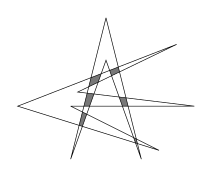
\includegraphics[width=6.4cm]{figures/2017-8-3B}
\end{center}

\itC Данная задача является обобщением \hyperref[float-ptb]{пункта B}. Из совершенно аналогичных соображений получаем ответ~--- от 3 до $m \cdot n$ углов.

\end{itemize}
